\chapter{System Design}
\label{chapter:design}

\section{Overview}
    \begin{table}[h]
    \centering
    % [] ��ܦb list of tables ����r
    % {} ��ܦb����W�誺��r
    \caption[Notations]{Notations}
    \label{table:notation}
    \begin{tabular}{lll}
    \toprule[1.1pt]
    Notation   & Description\\
    \midrule[1.1pt]
    \multirow{1}{*}{\(C_i\)} & Customer / User\\
    \midrule
    \multirow{1}{*}{\(Org_i\)} & Organization\\
    \midrule
    \multirow{1}{*}{\(RA\)} & Regulatory Authority\\
    \midrule
    \multirow{1}{*}{\(D_{ij}\)} & Data of \(C_i\) in \(Org_j\)\\
    \midrule
    \multirow{1}{*}{\({TSP}_i\)} & Third-party Service Provider\\
    \midrule
    \multirow{1}{*}{\({Acc}_{ij}\)} & \(Org_j\) Account of \(C_i\)\\
    \midrule
    \multirow{1}{*}{\({ID}_i\)} & Identification card number of \(C_i\)\\
    \midrule
    \multirow{1}{*}{\({Add}_i\)} & Ethereum address of i\\
    \midrule
    \multirow{1}{*}{\({Pri}_i\)} & Private key of \({Add}_i\)\\
    \midrule
    \multirow{1}{*}{\({DI}_i\)} & Digital Identity of \(C_i\)\\
    \midrule
    \multirow{1}{*}{\({R}_{ijk}\)} & Access right of \({TSP}_i\) to access \({Org}_j\) with \(C_k\) consent\\
    \midrule
    \multirow{1}{*}{\({ACMgr}_i\)} & Access Control Manager contract of \(C_i\) \\
    \midrule
    \multirow{1}{*}{\({OMgr}\)} & Organization contract \\
    \midrule
    \multirow{1}{*}{\({N}\)} & Nonce \\
    \bottomrule[1.1pt]
    \end{tabular}
    \end{table}
    \newpage    

    \begin{figure}[htb]
        \centering
        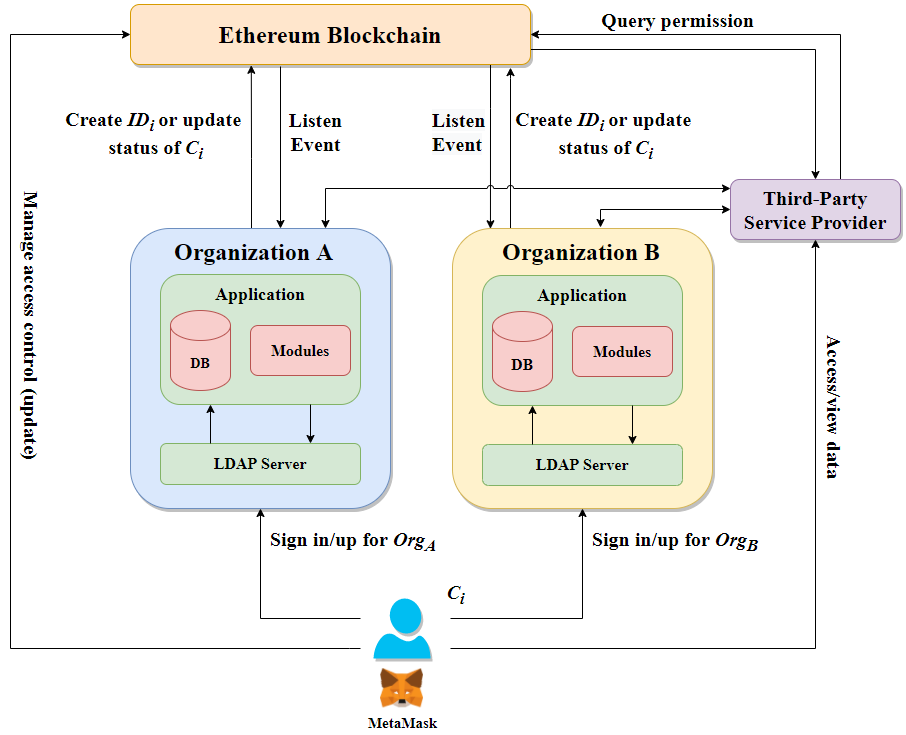
\includegraphics[height=!,width=1\linewidth,keepaspectratio=true]{figures/system_architecture.png}
        \caption{{\footnotesize System Architecture}}
        \label{fig:system_architecture}
    \end{figure}
    The architecture of our system is given in figure~\ref{fig:system_architecture}. Our proposed system solved the account integration and identity verification. And it can apply to various scenarios which need data sharing and distributed access control management such as open banking, medical records, and academic records. At the initial stage, each \(Org\) or \(TSP\) gets the exclusive \(Add\) and the corresponding \(Pri\) to take part in our open banking ecosystem. They must put the safety of \(Pri\) first and be careful; otherwise, identity theft may occur. There are several parties in our system: blockchain network, organization, third-party service provider, and user. The interpretation of these parties is stated as following:\par

    \begin{itemize}
        \item \textbf{Blockchain network:} The Ethereum blockchain network is used to store the user's \(DI\) and data access rights and deploy smart contracts, including identity creation and storage. Every node on blockchain has a copy of the ledger and ensures data on the blockchain cannot be tampered with. With decentralized technology, the management of data access rights doesn't have any governing authority to monitor. There have two kinds of contracts to realize that account integration and access manager, detailed in Sect.~\ref{chapter:implementation}.  
        \item \textbf{Organization:} A set of organizations within an ecosystem, identified by the \(Add\) and IP addresses. Each organization represents an independent system, it owns membership software that provides an organization with functionality such as storing and editing member information. The organization not only provides services to customers depend on applications, but also collects user data by using a database. In this paper, organizations provide an interface that users decide to share data.
        \begin{itemize}
            \item $DB_j = \{D_{1j}, D_{2j}, ..., D_{nj}\}$: Database of $Org_j$ is used to store customer data and only owner of data can decide which $TSP$ can access. 
            \item Because the organization $Org_j$ maintains membership software, it will provide the user $C_i$ a regular account $Acc_{ij}$. In the appilcation of $Org_j$, the user $C_i$ can access their data $D_{ij}$.
        \end{itemize}
        \item \textbf{Third-party service provider:} The third-party service provider can be any organization or entity that performs financial services to customer. In this paper, we assume that TSP doesn't manage membership software and they retrieve customer data through blockchain technology.
        \begin{itemize}
            \item The aim of the $TSP$ is to collect data of $C_i$ from organizations $\{Org_1, Org_2, ..., Org_n\}$ if the organization owns the data of $C_i$ and $TSP$ gets the permission.
            \item When the permission is revoked by triggering smart contract, the access data request is regarded as invalid even if the token exists and it is not out of date.
        \end{itemize}
        \item \textbf{User:} A user owns an organization account and wants to participate in our proposed system. After registering an organization account, the user first needs to pass identity card authentication. Due to the digital identity is unique and important on the smart contract, the organization takes responsibility for ensuring the correct identification card number and the safety of user's personal data. Besides, the user should generate the Ethereum account themself through Metamask.
    \end{itemize}

    \newpage    
\section{Scenario}
    \begin{figure}[htb]
        \centering
        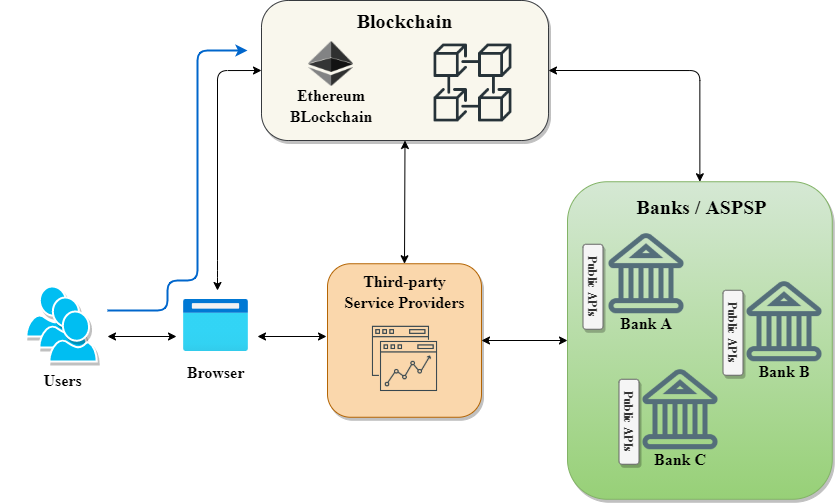
\includegraphics[height=!,width=1\linewidth,keepaspectratio=true]{figures/system architecture-banks.png}
        \caption{{\footnotesize Relation between open banking roles}}
        \label{fig:relation}
    \end{figure}
        From the user perspective, our proposed system provides a single digital identity \(DI_i\) and access control. The access control for data sharing is constructed using smart contracts. So when banks disclose user's personal data to TSP, banks must have the user's consent through call specific user's smart contract. \par
        In order to apply our proposed system to open banking ecosystem, we have three clearly defined roles: Customer (User), Financial institution, and Third-party services provider. Figure~\ref{fig:relation} gives an overview of our proposed system. It shows the relation between these roles and includes workflows, detailed in Sect.~\ref{ssec:workflow} Each customer interacts with Blockchain by using MetaMask, they not only login with MetaMask but also manage their own access manager contract. That's why customers can allow the specific party to access their data.\par
        The user can specify the data attribute, source, destination through the smart contract to decentralized access control. And the user also can revoke access rights while he/she doesn't need the service that TSP provides.\par
        
\section{Workflow} \label{ssec:workflow}
    \subsection{Identity verification}
    \begin{figure}[htb]
        \centering
        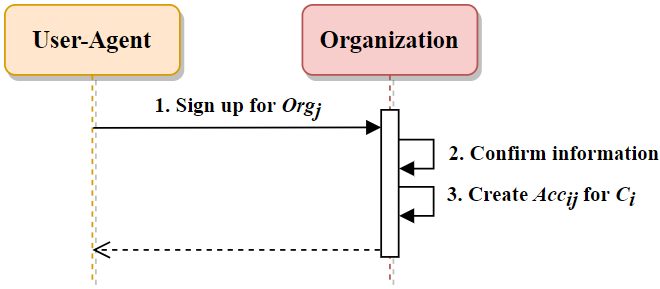
\includegraphics[height=!,width=0.8\linewidth,keepaspectratio=true]{figures/account_creation.png}
        \caption{{\footnotesize Account creation flow}}
        \label{fig:accountCreation}
    \end{figure}
    User registration is commonly used by many companies or any online service which record user data. Although in recent years there has been an increase in social login, the sign-up for social media is still necessary. Figure~\ref{fig:accountCreation} shows the flow for the user who visits the application (e.g., website of a bank) completes a signup form as shown in Table~\ref{table:signup}. The identification card number of the form is especially important for identity because it can be used to establish a digital identity on the blockchain. In this paper, we assume every organization should have its own membership software such as LDAP for users.
    \begin{table}[h]
    \centering
    % [] ��ܦb list of tables ����r
    % {} ��ܦb����W�誺��r
    \caption[Sign-up form used in each organization]{Sign-up form used in each organization}
    \label{table:signup}
    \begin{tabular}{lll}
    \toprule[1.1pt]
    Fields   & Description & required\\
    \midrule[1.1pt]
    \multirow{1}{*}{username} & Username as login account & Yes\\
    \midrule
    \multirow{1}{*}{password} & The password of the account & Yes \\
    \midrule
    \multirow{1}{*}{email} & User's email & No \\
    \midrule
    \multirow{1}{*}{phone} & User's phone & No \\
    \midrule
    \multirow{1}{*}{id card number} & Identification card number & No \\
    \bottomrule[1.1pt]
    \end{tabular}
    \end{table}
    \begin{figure}[htb]
        \centering
        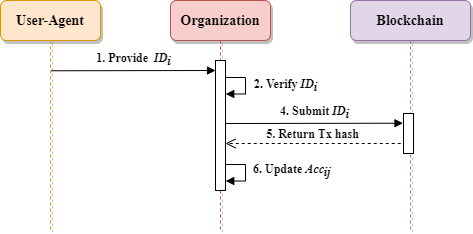
\includegraphics[height=!,width=0.8\linewidth,keepaspectratio=true]{figures/identity_verification.png}
        \caption{{\footnotesize Identity verification flow}}
        \label{fig:identityVerification}
    \end{figure}
    


    \newpage
    \subsection{Account binding}
    \begin{figure}[htb]
        \centering
        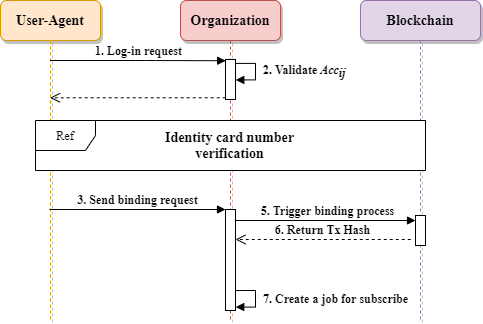
\includegraphics[height=!,width=0.8\linewidth,keepaspectratio=true]{figures/account_binding.png}
        \caption{{\footnotesize Account binding flow}}
        \label{fig:accountBinding}
    \end{figure}

    \newpage
    \subsection{Third-party login with Ethereum account}
    \begin{figure}[htb]
        \centering
        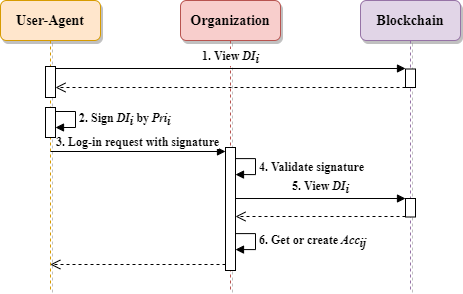
\includegraphics[height=!,width=0.8\linewidth,keepaspectratio=true]{figures/Third_party_login.png}
        \caption{{\footnotesize Third-party login flow}}
        \label{fig:thirdPartyLogin}
    \end{figure}


    \newpage
    \subsection{Data sharing}
    \begin{figure}[htb]
        \centering
        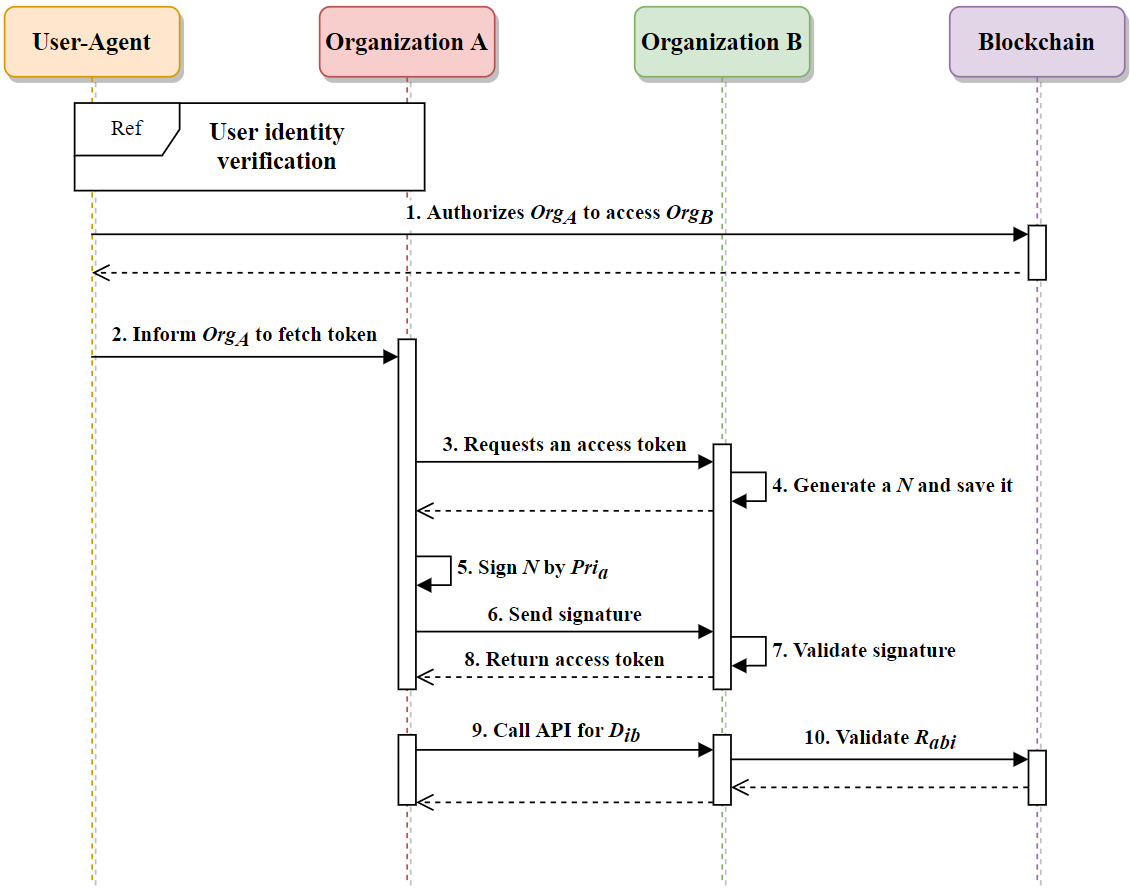
\includegraphics[height=!,width=1\linewidth,keepaspectratio=true]{figures/data_sharing.png}
        \caption{{\footnotesize Date Sharing flow}}
        \label{fig:dataSharing}
    \end{figure}

    \newpage